% interpolation_nncn - the process. Built by ../../documenting, which generates generated/*.tex and
% generated/*.csv from the repository first (options, methods, settings, measurements, version):
% only the explanations below are written by hand.
\documentclass[11pt,a4paper]{article}
\usepackage[T1]{fontenc}
\usepackage{lmodern}
\usepackage[margin=2.2cm]{geometry}
\usepackage{xcolor}
\usepackage{booktabs}
\usepackage{array}
\usepackage{longtable}
\usepackage{tabularx}
\usepackage{tikz}
\usetikzlibrary{arrows.meta,positioning,fit,backgrounds}
\usepackage{pgfplots}
\pgfplotsset{compat=1.18}
\usepackage{pgfplotstable}
\usepackage{newunicodechar}
\newunicodechar{≤}{\ensuremath{\le}}
\newunicodechar{≥}{\ensuremath{\ge}}
\newunicodechar{→}{\ensuremath{\to}}
\newunicodechar{×}{\ensuremath{\times}}
\newunicodechar{−}{\ensuremath{-}}
\newunicodechar{†}{\dag}
\newunicodechar{‡}{\ddag}
\newunicodechar{▊}{\rule{0.6em}{0.8em}}
\usepackage[hidelinks]{hyperref}
\urlstyle{same}

\input{generated/version.tex}
% generated table rows: TeX's primitive \input (LaTeX's own is protected, so a \bottomrule after it
% inside a longtable fails with "Misplaced \noalign")
\makeatletter
\newcommand{\tablerows}[1]{\@@input #1 }
\makeatother

\definecolor{step}{HTML}{DCEBFA}
\definecolor{background}{HTML}{FCE9D2}
\definecolor{state}{HTML}{E2F2DC}

\title{\texttt{interpolation\_nncn} -- the process\\[0.4em]
  \large how a film becomes a smoother one, and why it is built this way}
\author{movies\_management}
\date{built from commit \documentversion}

\begin{document}
\maketitle

\noindent\fbox{\parbox{\dimexpr\linewidth-2\fboxsep}{\small
\textbf{How to read this document.} Section~\ref{sec:overview} is for everyone: what the script
does and why it can be trusted with a long run. Sections~\ref{sec:running}--\ref{sec:measurements}
are the technical part. Every table and chart is \emph{generated} from the repository when the PDF
is built (the commit is on the title), so they match the scripts of that commit; only the
explanations are written by hand.}}

\tableofcontents

%------------------------------------------------------------------------------------------------
\section{Overview}\label{sec:overview}

\texttt{interpolation\_nncn} takes a film (for example 23.976 frames per second) and lets a neural
network calculate the frames \emph{between} the existing ones, so the result has twice as many
(47.952 fps) and motion looks smoother. A 4K film has about 170\,000 frames; processing them all at
once would need several terabytes of space and a day without any interruption. The script
therefore works in \textbf{chunks of about one minute}: each chunk is processed on its own, checked,
and marked as finished. This gives the properties the rest of the design follows from:

\begin{itemize}
  \item \textbf{A run can stop at any moment} (Ctrl+C, a reboot, a power cut) and the next run
    \emph{resumes}: finished chunks are skipped, an unfinished one is redone.
  \item \textbf{The space needed is that of one chunk}, not of the film: frames are deleted as soon
    as nothing needs them any more.
  \item \textbf{Slow work runs alongside}: the final encode and the quality check (VMAF) of a chunk
    run in the background while the next chunk is prepared.
  \item \textbf{Everything is measured}: each step's start and end (\texttt{timeline.csv}) and the
    machine's load (\texttt{metrics.csv}) are recorded, so every change can be checked against real
    runs (Section~\ref{sec:measurements}).
\end{itemize}

%------------------------------------------------------------------------------------------------
\section{The process}\label{sec:process}

Figure~\ref{fig:pipeline} shows one run. The steps on the left happen once per film, the box in the
middle once per chunk; the orange steps run in the background, overlapping the next chunk.

\begin{figure}[ht]
\centering
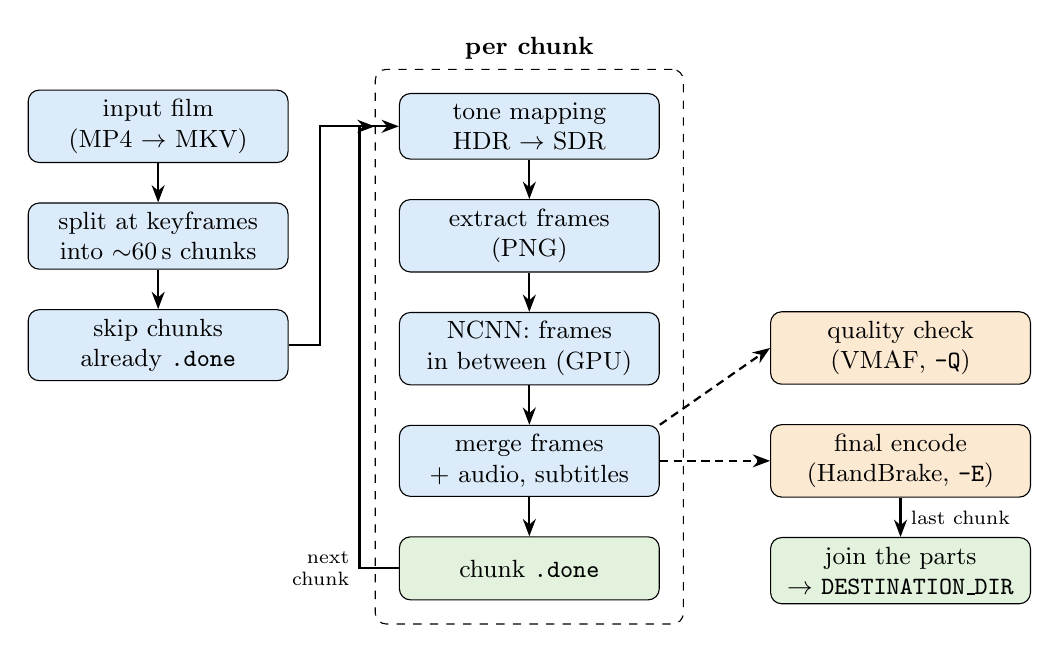
\begin{tikzpicture}[
  node distance=5mm and 9mm,
  every node/.style={font=\small},
  box/.style={draw, rounded corners, fill=step, align=center, minimum width=33mm, minimum height=8mm},
  bg/.style={box, fill=background},
  done/.style={box, fill=state},
  arrow/.style={-{Stealth[length=2.2mm]}, thick}]
  % once per film
  \node[box] (input) {input film\\(MP4 $\to$ MKV)};
  \node[box, below=of input] (split) {split at keyframes\\into $\sim$60\,s chunks};
  \node[box, below=of split] (resume) {skip chunks\\already \texttt{.done}};
  % per chunk
  \node[box, right=14mm of input] (tone) {tone mapping\\HDR $\to$ SDR};
  \node[box, below=of tone] (extract) {extract frames\\(PNG)};
  \node[box, below=of extract] (ncnn) {NCNN: frames\\in between (GPU)};
  \node[box, below=of ncnn] (merge) {merge frames\\+ audio, subtitles};
  \node[done, below=of merge] (mark) {chunk \texttt{.done}};
  \begin{scope}[on background layer]
    \node[draw, dashed, rounded corners, inner sep=3mm, fit=(tone)(mark), label={[font=\small\bfseries]above:per chunk}] (chunk) {};
  \end{scope}
  % background
  \node[bg, right=14mm of merge] (encode) {final encode\\(HandBrake, \texttt{-E})};
  \node[bg, above=of encode] (vmaf) {quality check\\(VMAF, \texttt{-Q})};
  \node[done, below=of encode] (join) {join the parts\\$\to$ \texttt{DESTINATION\_DIR}};
  \draw[arrow] (input) -- (split);
  \draw[arrow] (split) -- (resume);
  \draw[arrow] (resume.east) -- ++(4mm,0) |- (tone.west);
  \draw[arrow] (tone) -- (extract);
  \draw[arrow] (extract) -- (ncnn);
  \draw[arrow] (ncnn) -- (merge);
  \draw[arrow] (merge) -- (mark);
  \draw[arrow, densely dashed] (merge) -- (encode);
  \draw[arrow, densely dashed] (merge.north east) -- (vmaf.west);
  \draw[arrow] (encode) -- node[right, font=\scriptsize] {last chunk} (join);
  \draw[arrow] (mark.west) -- ++(-5mm,0) node[left, font=\scriptsize, align=right] {next\\chunk} |- (chunk.west |- tone);
\end{tikzpicture}
\caption{One run of \texttt{interpolation\_nncn}. Dashed: started in the background.}
\label{fig:pipeline}
\end{figure}

Two details make the chunk loop fast and safe:
\begin{description}
  \item[NCNN starts before the extraction ends.] It is paused (SIGSTOP) when it comes too close to
    the frames extracted so far and continues (SIGCONT) when the extraction is ahead again
    (\texttt{NCNN\_EXTRACTION\_MARGIN}, Section~\ref{sec:settings}).
  \item[Input frames are deleted on a provable rule.] A frame is removed only when every output
    frame that needs it is finished -- read from NCNN's own log, in order, so outputs finished out
    of order never lose an input.
\end{description}

%------------------------------------------------------------------------------------------------
\section{Running it}\label{sec:running}

\subsection{Options}
Generated from \texttt{interpolation\_nncn -h}.

\begin{small}
\begin{longtable}{@{}l p{0.82\linewidth}@{}}
\toprule
\textbf{option} & \textbf{meaning} \\
\midrule
\endhead
\tablerows{generated/options.tex}
\bottomrule
\end{longtable}
\end{small}

\subsection{Methods (\texttt{-N})}
Generated from the method list of \texttt{-h}; ``no'' means rejected by the script for now.

\begin{small}
\begin{longtable}{@{}l l p{0.38\linewidth} p{0.36\linewidth}@{}}
\toprule
\textbf{method} & \textbf{supported} & \textbf{what it does} & \textbf{project} \\
\midrule
\endhead
\tablerows{generated/methods.tex}
\bottomrule
\end{longtable}
\end{small}

%------------------------------------------------------------------------------------------------
\section{Settings}\label{sec:settings}

Settings are environment variables with a default (\texttt{NAME="\$\{NAME:-default\}"}). The
description is the comment above each one in the code -- a setting without a comment stops the
build. \emph{-S} tells whether a service run (\texttt{-S}) receives the value: a service starts with
a clean environment, so a setting it does not receive falls back to its default there.

\begin{small}
\begin{longtable}{@{}>{\raggedright}p{0.3\linewidth} >{\raggedright}p{0.14\linewidth} l p{0.42\linewidth}@{}}
\toprule
\textbf{setting} (file) & \textbf{default} & \textbf{-S} & \textbf{description} \\
\midrule
\endhead
\tablerows{generated/settings.tex}
\bottomrule
\end{longtable}
\end{small}

%------------------------------------------------------------------------------------------------
\section{Measurements}\label{sec:measurements}

Average time per chunk and step, generated from the ``State over time'' table of
\texttt{README.md} (4K HDR, about 50 chunks per column; empty: not measured then). The last column is
a different film with the same options, so it shows the trend rather than an exact comparison.
Background steps overlap the next chunk, so the steps do not add up to the chunk total.

\begin{figure}[ht]
\centering
\pgfplotstableread[col sep=semicolon]{generated/state_over_time.csv}\statetable
\pgfplotstablegetrowsof{\statetable}
\pgfmathtruncatemacro{\lastrow}{\pgfplotsretval - 1}
\begin{tikzpicture}
\begin{axis}[
  xbar, width=0.8\linewidth, height=0.85\linewidth,
  bar width=3pt, enlarge y limits=0.06,
  xmin=0, xlabel={seconds per chunk},
  % ticks for every row: "data" would follow the first column, which has empty (nan) rows
  ytick={0,...,\lastrow}, y dir=reverse,
  yticklabels from table={\statetable}{step},
  yticklabel style={font=\small, align=right, text width=32mm},
  legend style={at={(0.5,-0.12)}, anchor=north, font=\small, legend columns=2},
  legend cell align=left, bar width=4pt,
  unbounded coords=jump]
  \addplot table[x=c1, y expr=\coordindex] {\statetable};
  \addplot table[x=c2, y expr=\coordindex] {\statetable};
  \addplot table[x=c3, y expr=\coordindex] {\statetable};
  \addplot table[x=c4, y expr=\coordindex] {\statetable};
  \input{generated/state_over_time_legend.tex}
\end{axis}
\end{tikzpicture}
\caption{Time per chunk over the optimisation rounds (from \texttt{README.md}).}
\label{fig:state}
\end{figure}

%------------------------------------------------------------------------------------------------
\section{Design rules}\label{sec:rules}

The rules the script follows, and this document with it; they are meant to carry over to other
repositories.
\begin{enumerate}
  \item \textbf{Check before starting.} Tools, space, memory and the input are checked first; a run
    that cannot finish does not start.
  \item \textbf{Every result is either finished or absent.} A chunk is marked \texttt{.done} only after
    its checks; anything unfinished is redone, never trusted.
  \item \textbf{Measure, then decide.} Each change is checked against real runs; the measurements
    stay in the repository (\texttt{README.md}) and feed this document.
  \item \textbf{One source for every fact.} Options, settings and measurements are read from where
    they are defined; a second, hand-written copy would drift away.
  \item \textbf{Security and the least privilege.} A background run (\texttt{-S}) is a systemd
    service that runs as the user, not as root, optionally with a memory limit (\texttt{-M}).
\end{enumerate}

%------------------------------------------------------------------------------------------------
\appendix
\section{How this document is built}
\texttt{./documenting} (in the repository) checks the tools and LaTeX packages it needs, copies
\texttt{docs/interpolation/} into a work directory under \texttt{tmp/}, generates the tables and the
chart data from the repository, runs \texttt{latexmk}, and writes the PDF to \texttt{tmp/} (\texttt{-o}
elsewhere; \texttt{-k} keeps the work directory). The PDF is not committed: it can always be built
again from its commit.

\end{document}
